% =====================================================================================
% The Quantum Fourier Transform - explained for first-year engineering students
% Build:  python make_figures.py   (needs cudaq, numpy, matplotlib)
%         latexmk -pdf qft_lecture.tex
% =====================================================================================
\documentclass[aspectratio=169,11pt]{beamer}
\usepackage[T1]{fontenc}
\usepackage{lmodern}
\usepackage{amsmath,amssymb}
\usepackage{braket}
\usepackage{graphicx}
\usepackage{booktabs}
\usepackage{array}
\usepackage{tikz}
\usepackage{quantikz}
\usepackage{listings}
\graphicspath{{figures/}}
\newcommand{\fidfifteen}{1.000000000000}
\newcommand{\maxerrfifteen}{4.6e-16}

\newcommand{\qftfiverows}{%
$|000\rangle$ & 0 & $+0.3536$ & $+0.0000$ & $0^\circ$ & 0.1250 \\
$|001\rangle$ & 1 & $-0.2500$ & $-0.2500$ & $225^\circ$ & 0.1250 \\
$|010\rangle$ & 2 & $+0.0000$ & $+0.3536$ & $90^\circ$ & 0.1250 \\
$|011\rangle$ & 3 & $+0.2500$ & $-0.2500$ & $315^\circ$ & 0.1250 \\
$|100\rangle$ & 4 & $-0.3536$ & $+0.0000$ & $180^\circ$ & 0.1250 \\
$|101\rangle$ & 5 & $+0.2500$ & $+0.2500$ & $45^\circ$ & 0.1250 \\
$|110\rangle$ & 6 & $+0.0000$ & $-0.3536$ & $270^\circ$ & 0.1250 \\
$|111\rangle$ & 7 & $-0.2500$ & $+0.2500$ & $135^\circ$ & 0.1250 \\
}

\newcommand{\periodicrows}{%
0 & $+0.500+0.000i$ & 0.250 & $0^\circ$ \\
4 & $+0.000+0.500i$ & 0.250 & $90^\circ$ \\
8 & $-0.500+0.000i$ & 0.250 & $180^\circ$ \\
12 & $+0.000-0.500i$ & 0.250 & $270^\circ$ \\
}


% ---- colours and look ---------------------------------------------------------------
\definecolor{qblue}{HTML}{2A78D6}
\definecolor{qdark}{HTML}{1C5CAB}
\definecolor{qorange}{HTML}{EB6834}
\definecolor{qaqua}{HTML}{1BAF7A}
\definecolor{qink}{HTML}{0B0B0B}
\definecolor{qgrey}{HTML}{52514E}
\definecolor{qlight}{HTML}{EEF4FC}
\setbeamercolor{structure}{fg=qdark}
\setbeamercolor{frametitle}{fg=qdark}
\setbeamercolor{title}{fg=qdark}
\setbeamercolor{normal text}{fg=qink}
\setbeamercolor{block title}{bg=qblue,fg=white}
\setbeamercolor{block body}{bg=qlight,fg=qink}
\setbeamercolor{block title example}{bg=qaqua,fg=white}
\setbeamercolor{block body example}{bg=qaqua!10,fg=qink}
\setbeamercolor{block title alerted}{bg=qorange,fg=white}
\setbeamercolor{block body alerted}{bg=qorange!10,fg=qink}
\setbeamertemplate{blocks}[rounded][shadow=false]
\setbeamertemplate{navigation symbols}{}
\setbeamertemplate{itemize items}[circle]
\setbeamertemplate{enumerate items}[default]
\setbeamerfont{frametitle}{size=\large,series=\bfseries}
% =====================================================================================
% SILICO FELLER branding for the beamer lecture decks (16:9).
% \input this file in the preamble of every presentations/<algorithm>_source/<algorithm>_lecture.tex,
% after graphicx is loaded and the colours/fonts are set. It is the "slide master":
%   * the official logo (assets/branding/silico_feller_logo.png, unmodified, aspect ratio kept)
%     is drawn at the top-right of EVERY slide through the background template, so new or
%     re-ordered slides get it automatically;
%   * the frame-title box is narrowed on the right so titles wrap before they can reach the logo.
% =====================================================================================
\makeatletter
\newcommand{\sflogofile}{../../assets/branding/silico_feller_logo.png}
\newlength{\sflogoheight}\setlength{\sflogoheight}{5.4mm}   % logo height on the slide (width follows the aspect ratio)
\newlength{\sflogomargin}\setlength{\sflogomargin}{2.5mm}   % distance from the top and right paper edges
\newlength{\sflogoreserve}\setlength{\sflogoreserve}{2.6cm} % horizontal space kept free for the logo in the title row

% logo on every slide (background layer: never covers slide content)
\setbeamertemplate{background}{%
  \vbox to \paperheight{%
    \vskip\sflogomargin
    \hbox to \paperwidth{\hfill\includegraphics[height=\sflogoheight]{\sflogofile}\hskip\sflogomargin}%
    \vfill}}

% frame title: same look as beamer's default, but it stops \sflogoreserve before the right edge
\setbeamertemplate{frametitle}{%
  \ifbeamercolorempty[bg]{frametitle}{}{\nointerlineskip}%
  \begin{beamercolorbox}[sep=0.3cm,left,wd=\paperwidth]{frametitle}%
    \usebeamerfont{frametitle}%
    \vbox{}\vskip-1ex%
    \parbox[t]{\dimexpr\paperwidth-0.6cm-\sflogoreserve\relax}{\raggedright
      \strut\insertframetitle\strut\par
      \ifx\insertframesubtitle\@empty\else
        {\usebeamerfont{framesubtitle}\usebeamercolor[fg]{framesubtitle}\insertframesubtitle\strut\par}%
      \fi}%
    \vskip-1ex%
    \vskip-.3cm%
  \end{beamercolorbox}}
\makeatother
   % SILICO FELLER logo on every slide
\setbeamertemplate{footline}{%
  \leavevmode\hbox{\begin{beamercolorbox}[wd=\paperwidth,ht=2.4ex,dp=1ex,leftskip=0.4cm,rightskip=0.4cm]{normal text}%
    \color{qgrey}\tiny The Quantum Fourier Transform\ \ $\cdot$\ \ \insertsectionhead\hfill\insertframenumber\,/\,\inserttotalframenumber
  \end{beamercolorbox}}}
\newcommand{\hl}[1]{{\color{qorange}\textbf{#1}}}
\newcommand{\key}[1]{{\color{qdark}\textbf{#1}}}

\lstset{language=Python, basicstyle=\ttfamily\scriptsize, keywordstyle=\color{qdark}\bfseries,
  commentstyle=\color{qgrey}\itshape, stringstyle=\color{qorange}, showstringspaces=false,
  frame=single, rulecolor=\color{qblue!40}, backgroundcolor=\color{qlight}, columns=fullflexible}

\title{The Quantum Fourier Transform}
\subtitle{From sound waves to quantum circuits --- explained step by step}
\author{CUDA-Q Quantum Algorithm Benchmarking Suite}
\date{For first-year engineering students}

\begin{document}

% =====================================================================================
\section{Introduction}
\begin{frame}
  \titlepage
  \centering\small\color{qgrey}
  All quantum results in these slides were computed with NVIDIA CUDA-Q and checked against NumPy.
\end{frame}

\begin{frame}{What you will learn today}
  \begin{columns}[T]
    \begin{column}{0.55\textwidth}
      \begin{enumerate}
        \item Why engineers love the \key{Fourier transform}
        \item The math toolkit: \key{complex numbers}, roots of unity, binary fractions
        \item \key{Qubits} in ten minutes
        \item The \key{Quantum Fourier Transform (QFT)}: definition and small examples
        \item How to \key{build the QFT circuit} from simple gates
        \item Examples: \key{periodic signals}, peaks and leakage (with real simulation results)
        \item Where the QFT is used, its limits, and how to run it in \key{CUDA-Q}
      \end{enumerate}
    \end{column}
    \begin{column}{0.42\textwidth}
      \begin{block}{You only need}
        \begin{itemize}
          \item school algebra (powers, sums)
          \item vectors and matrices (multiplying a matrix by a vector)
          \item a little trigonometry ($\sin$, $\cos$)
        \end{itemize}
        Everything else is explained on the way.
      \end{block}
    \end{column}
  \end{columns}
\end{frame}

% =====================================================================================
\section{Part 1: Why Fourier?}
\begin{frame}{Every signal is a sum of waves}
  \centering
  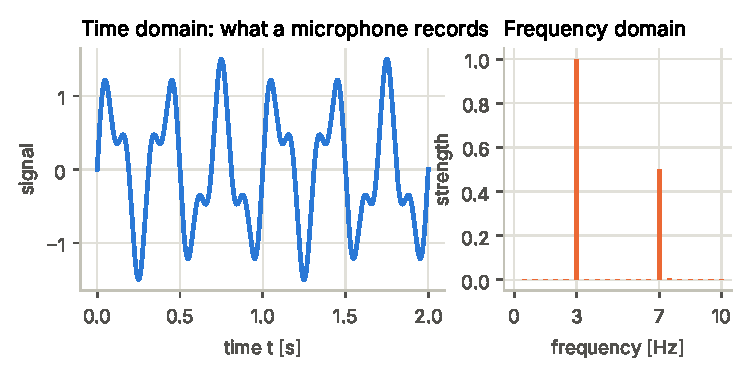
\includegraphics[width=0.74\textwidth]{sound}\\[0mm]
  \raggedright
  The signal on the left looks complicated, but it is just
  \[ s(t) = \underbrace{\sin(2\pi\cdot 3\,t)}_{3\text{ Hz wave}} + \underbrace{0.5\,\sin(2\pi\cdot 7\,t)}_{7\text{ Hz wave}} . \]
  The \key{Fourier transform} finds these ingredients: \hl{which frequencies, and how strong}.
\end{frame}

\begin{frame}{Fourier analysis is everywhere in engineering}
  \begin{columns}[T]
    \begin{column}{0.48\textwidth}
      \begin{itemize}
        \item \key{Audio}: MP3 and equalisers work on frequencies
        \item \key{Images}: JPEG stores frequency coefficients
        \item \key{Telecom}: Wi-Fi, 4G/5G (OFDM) send data on many frequencies at once
        \item \key{Medicine}: MRI images are reconstructed with Fourier transforms
        \item \key{Mechanics}: vibration analysis finds the resonance frequencies of bridges, engines, wings
      \end{itemize}
    \end{column}
    \begin{column}{0.48\textwidth}
      \begin{block}{The common idea}
        Change the point of view:\\[1mm]
        \centering
        \textbf{time / position} $\longrightarrow$ \textbf{frequency}\\[1mm]
        \raggedright
        Some questions are hard in one view and easy in the other --- for example
        \hl{``what is the period of this signal?''}
      \end{block}
      \vspace{2mm}
      The quantum computer uses exactly this trick to find hidden periods (Shor's factoring algorithm).
    \end{column}
  \end{columns}
\end{frame}

\begin{frame}{The Discrete Fourier Transform (DFT)}
  A computer stores a signal as $M$ samples $x_0, x_1, \dots, x_{M-1}$. The DFT turns them into $M$ frequency
  coefficients:
  \begin{block}{Discrete Fourier Transform}
    \[ X_k = \sum_{n=0}^{M-1} x_n\, e^{-2\pi i\, kn/M}, \qquad k = 0, 1, \dots, M-1 . \]
  \end{block}
  \begin{itemize}
    \item $k$ = frequency index: ``how many full oscillations fit into the $M$ samples''
    \item $e^{-2\pi i kn/M}$ is a wave written with complex numbers (next part explains why)
    \item $|X_k|$ = how strongly frequency $k$ is present in the signal
  \end{itemize}
\end{frame}

\begin{frame}{Example: the DFT finds the period}
  \centering
  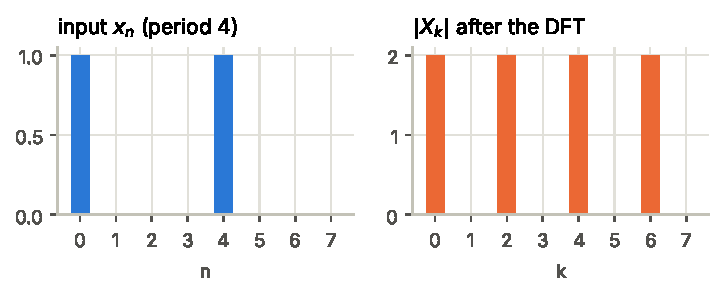
\includegraphics[width=0.66\textwidth]{dft_periodic}\\[1mm]
  \raggedright
  \begin{columns}[T]
    \begin{column}{0.48\textwidth}
      A spike every $r = 4$ samples. Only $n = 0, 4$ contribute and $e^{-2\pi i\cdot 4k/8} = (-1)^k$, so
      \[ X_k = 1 + (-1)^k = \begin{cases} 2 & k \text{ even}\\ 0 & k \text{ odd}\end{cases} \]
    \end{column}
    \begin{column}{0.44\textwidth}
      \begin{alertblock}{Remember this pattern}
        Period $r$ in the input $\Rightarrow$ peaks at multiples of $M/r$ in the output (here $8/4 = 2$: $k = 0, 2, 4, 6$).
      \end{alertblock}
    \end{column}
  \end{columns}
\end{frame}

\begin{frame}{How expensive is a Fourier transform?}
  \begin{columns}[T]
    \begin{column}{0.5\textwidth}
      \begin{itemize}
        \item Direct formula: $M$ outputs $\times$ $M$ terms = $M^2$ multiplications
        \item \key{Fast Fourier Transform (FFT)}, 1965: only about $M\log_2 M$
      \end{itemize}
      \vspace{2mm}
      \begin{tabular}{lrr}
        \toprule
        $M$ & $M^2$ & $M\log_2 M$\\
        \midrule
        $1\,024$ & $10^6$ & $10^4$\\
        $10^6$ & $10^{12}$ & $2\times 10^7$\\
        \bottomrule
      \end{tabular}
    \end{column}
    \begin{column}{0.47\textwidth}
      \begin{block}{The quantum idea (preview)}
        $n$ qubits hold $M = 2^n$ numbers at once.\\[1mm]
        The QFT transforms all of them with only about $n^2/2$ simple operations.\\[1mm]
        For $n = 30$: $M \approx 10^9$ numbers, but only $\approx 480$ gates.
      \end{block}
      \vspace{1mm}
      \hl{But}: we cannot simply read out all $M$ results --- we will see why and how algorithms work around it.
    \end{column}
  \end{columns}
\end{frame}

% =====================================================================================
\section{Part 2: Complex numbers toolkit}
\begin{frame}{Complex numbers and Euler's formula}
  \begin{columns}[c]
    \begin{column}{0.56\textwidth}
      \begin{itemize}
        \item A complex number $z = a + ib$ with $i^2 = -1$ is a point in the plane: real part $a$, imaginary part $b$.
        \item Length (magnitude): $|z| = \sqrt{a^2 + b^2}$
        \item \key{Euler's formula} --- the most useful identity of this course:
      \end{itemize}
      \begin{block}{}
        \[ e^{i\varphi} = \cos\varphi + i\,\sin\varphi \]
      \end{block}
      $e^{i\varphi}$ is the point on the \hl{unit circle} at angle $\varphi$. Every complex number is
      $z = |z|\,e^{i\varphi}$: a length and a direction (``phase'').
    \end{column}
    \begin{column}{0.4\textwidth}
      \centering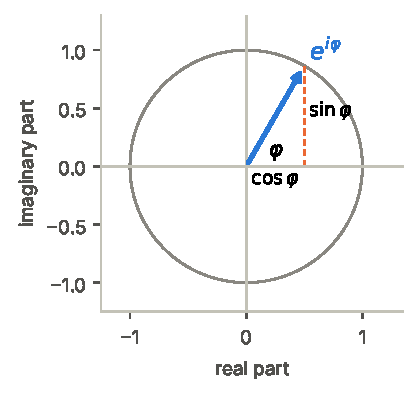
\includegraphics[width=\textwidth]{euler}
    \end{column}
  \end{columns}
\end{frame}

\begin{frame}{Multiplying phases = adding angles}
  \begin{columns}[T]
    \begin{column}{0.5\textwidth}
      \[ e^{i\alpha}\cdot e^{i\beta} = e^{i(\alpha+\beta)} \]
      Multiplying by $e^{i\beta}$ \key{rotates} a point by the angle $\beta$.
      \vspace{3mm}
      \begin{block}{Values to remember}
        \centering
        \begin{tabular}{cc}
          $e^{i\cdot 0} = 1$ & $e^{i\pi/2} = i$\\[1mm]
          $e^{i\pi} = -1$ & $e^{i 3\pi/2} = -i$\\[1mm]
          \multicolumn{2}{c}{$e^{2\pi i} = 1$}
        \end{tabular}
      \end{block}
    \end{column}
    \begin{column}{0.46\textwidth}
      \begin{alertblock}{The key fact for the QFT}
        A full turn changes nothing:
        \[ e^{2\pi i\,k} = 1 \quad\text{for every integer } k . \]
        So in $e^{2\pi i\,(\text{number})}$ only the \hl{fractional part} of the number matters:
        \[ e^{2\pi i\cdot 2.25} = e^{2\pi i\cdot 0.25} = i . \]
      \end{alertblock}
    \end{column}
  \end{columns}
\end{frame}

\begin{frame}{Roots of unity: equally spaced points on the circle}
  \begin{columns}[c]
    \begin{column}{0.5\textwidth}
      Define
      \[ \omega = e^{2\pi i/M} . \]
      Its powers $\omega^0, \omega^1, \dots, \omega^{M-1}$ are $M$ equally spaced points on the unit circle, and
      $\omega^M = 1$.\\[2mm]
      \begin{itemize}
        \item $M = 2$: $\omega = -1$
        \item $M = 4$: $\omega = i$
        \item $M = 8$: $\omega = e^{i\pi/4}$ (45$^\circ$ steps)
      \end{itemize}
      The QFT on $n$ qubits uses $M = 2^n$.
    \end{column}
    \begin{column}{0.48\textwidth}
      \centering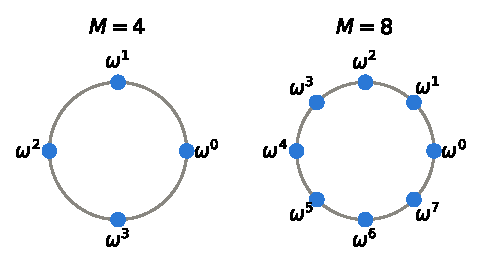
\includegraphics[width=\textwidth]{roots_of_unity}\\
      \small $\omega^k$ = point at angle $k\cdot 360^\circ/M$
    \end{column}
  \end{columns}
\end{frame}

\begin{frame}{Why peaks appear: arrows that cancel}
  \begin{columns}[c]
    \begin{column}{0.47\textwidth}
      \begin{block}{Sum of roots of unity}
        \[ \sum_{j=0}^{M-1} \omega^{jk} = \begin{cases} M & \text{if } k \text{ is a multiple of } M\\ 0 & \text{otherwise}\end{cases} \]
      \end{block}
      \small
      Proof (geometric series): for $\omega^k \ne 1$,
      $\sum_j (\omega^k)^j = \dfrac{1 - \omega^{kM}}{1-\omega^k} = \dfrac{1-1}{1-\omega^k} = 0$.\\[2mm]
      \normalsize
      Adding arrows head-to-tail: if they all point the same way they add up; if they are spread evenly around the
      circle they \hl{cancel}.
    \end{column}
    \begin{column}{0.5\textwidth}
      \centering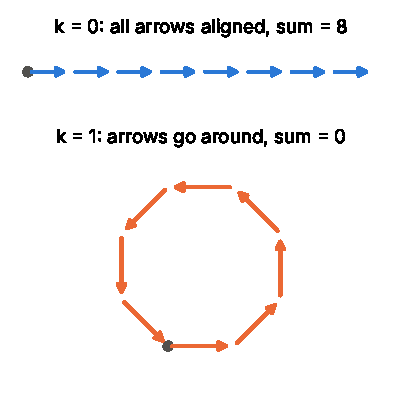
\includegraphics[height=0.68\textheight]{cancellation}\\
      \small $M = 8$: the arrows $\omega^{jk}$, $j = 0, \dots, 7$, added head-to-tail
    \end{column}
  \end{columns}
\end{frame}

\begin{frame}{Binary numbers and binary fractions}
  \begin{columns}[T]
    \begin{column}{0.48\textwidth}
      \key{Integers} with $n$ bits (we write the most significant bit first):
      \[ x = x_1x_2\dots x_n = x_1 2^{n-1} + \dots + x_n 2^0 \]
      Example: $5 = 101_2 = 4 + 0 + 1$.\\[3mm]
      \key{Binary fractions}:
      \[ 0.x_1x_2\dots x_m = \frac{x_1}{2} + \frac{x_2}{4} + \dots + \frac{x_m}{2^m} \]
    \end{column}
    \begin{column}{0.48\textwidth}
      \begin{tabular}{ll}
        \toprule
        binary & decimal\\
        \midrule
        $0.1_2$ & $1/2 = 0.5$\\
        $0.01_2$ & $1/4 = 0.25$\\
        $0.11_2$ & $3/4 = 0.75$\\
        $0.101_2$ & $5/8 = 0.625$\\
        \bottomrule
      \end{tabular}
      \vspace{2mm}
      \begin{block}{Shifting the point}
        Dividing by 2 moves the binary point one place left:
        $5/2 = 10.1_2$, $\ 5/4 = 1.01_2$, $\ 5/8 = 0.101_2$.
      \end{block}
    \end{column}
  \end{columns}
\end{frame}

% =====================================================================================
\section{Part 3: Qubits in ten minutes}
\begin{frame}{Bit vs. qubit}
  \begin{columns}[T]
    \begin{column}{0.46\textwidth}
      A classical \key{bit} is 0 or 1.\\[2mm]
      A \key{qubit} is a unit vector of two complex numbers:
      \[ \ket{0} = \begin{pmatrix}1\\0\end{pmatrix}, \quad \ket{1} = \begin{pmatrix}0\\1\end{pmatrix} \]
      \[ \ket{\psi} = \alpha\ket{0} + \beta\ket{1} = \begin{pmatrix}\alpha\\ \beta\end{pmatrix} \]
      with $|\alpha|^2 + |\beta|^2 = 1$.
      $\alpha, \beta$ are called \key{amplitudes}.
    \end{column}
    \begin{column}{0.44\textwidth}
      \begin{exampleblock}{Superposition}
        \[ \ket{+} = \tfrac{1}{\sqrt2}\big(\ket{0} + \ket{1}\big) \]
        is ``0 and 1 at the same time'' --- more precisely: a vector with two non-zero components.
      \end{exampleblock}
      \vspace{2mm}
      The notation $\ket{\cdot}$ (``ket'') just marks a column vector.
    \end{column}
  \end{columns}
\end{frame}

\begin{frame}{Measurement: amplitudes become probabilities}
  \begin{block}{Born rule}
    Measuring $\alpha\ket{0} + \beta\ket{1}$ gives 0 with probability $|\alpha|^2$ and 1 with probability $|\beta|^2$.
    Afterwards the qubit \emph{is} in the measured state.
  \end{block}
  \centering
  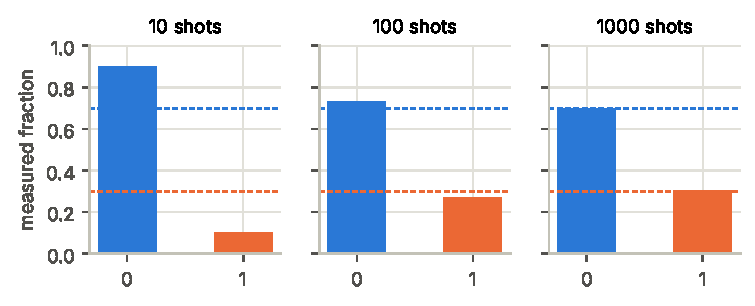
\includegraphics[width=0.85\textwidth]{measurement_shots}\\
  \raggedright\small
  A qubit with $|\alpha|^2 = 0.7$ measured 10, 100 and 1000 times (CUDA-Q). One \key{shot} gives one bit; the
  probabilities only appear after many shots (dashed lines: 0.7 and 0.3).
\end{frame}

\begin{frame}{The phase: invisible, but it matters}
  \begin{columns}[T]
    \begin{column}{0.5\textwidth}
      \[ \ket{+} = \tfrac{1}{\sqrt2}(\ket{0} + \ket{1}), \qquad \ket{-} = \tfrac{1}{\sqrt2}(\ket{0} - \ket{1}) \]
      Both give 50\,\% / 50\,\% when measured --- the minus sign (a \key{phase} $e^{i\pi}$) is invisible.\\[2mm]
      But after one more gate (the Hadamard $H$, next slide):
      \[ H\ket{+} = \ket{0}, \qquad H\ket{-} = \ket{1} \]
      Now the phase decides the result!
    \end{column}
    \begin{column}{0.46\textwidth}
      \begin{block}{Phase states}
        \[ \tfrac{1}{\sqrt2}\big(\ket{0} + e^{i\varphi}\ket{1}\big) \]
        All have 50/50 probabilities; they differ only in the angle $\varphi$ --- think of a \hl{clock hand}.\\[2mm]
        The QFT writes information into exactly these angles.
      \end{block}
    \end{column}
  \end{columns}
\end{frame}

\begin{frame}{Many qubits: $2^n$ amplitudes}
  \begin{itemize}
    \item $n$ qubits have $2^n$ basis states $\ket{x_1x_2\dots x_n}$, one for every $n$-bit number $x$:
      \[ \ket{\psi} = \sum_{x=0}^{2^n-1} \alpha_x \ket{x}, \qquad \sum_x |\alpha_x|^2 = 1 . \]
    \item Two qubits: $\ket{\psi} = \alpha_0\ket{00} + \alpha_1\ket{01} + \alpha_2\ket{10} + \alpha_3\ket{11}$
    \item Independent qubits combine with the \key{tensor product}: $(a\ket0 + b\ket1)\otimes(c\ket0 + d\ket1)
      = ac\ket{00} + ad\ket{01} + bc\ket{10} + bd\ket{11}$
    \item \key{Convention} in these slides (and in the CUDA-Q notebooks): qubit 1 (top wire) is the
      \hl{most significant bit} $x_1$.
  \end{itemize}
  \begin{alertblock}{Why simulation is hard}
    A classical computer must store all $2^n$ complex numbers: 16 bytes each, so $n = 30$ needs 17\,GB and $n = 50$
    needs 18 petabytes.
  \end{alertblock}
\end{frame}

\begin{frame}{Single-qubit gates are $2\times 2$ matrices}
  \begin{columns}[T]
    \begin{column}{0.32\textwidth}
      \begin{block}{NOT gate $X$}
        \[ X = \begin{pmatrix}0&1\\1&0\end{pmatrix} \]
        $X\ket0 = \ket1$, $X\ket1 = \ket0$
      \end{block}
    \end{column}
    \begin{column}{0.32\textwidth}
      \begin{block}{Hadamard $H$}
        \[ H = \tfrac{1}{\sqrt2}\begin{pmatrix}1&1\\1&-1\end{pmatrix} \]
        $H\ket0 = \ket+$, $H\ket1 = \ket-$
      \end{block}
    \end{column}
    \begin{column}{0.32\textwidth}
      \begin{block}{Phase gate $R_k$}
        \[ R_k = \begin{pmatrix}1&0\\0&e^{2\pi i/2^k}\end{pmatrix} \]
        turns the $\ket1$ part by $360^\circ/2^k$
      \end{block}
    \end{column}
  \end{columns}
  \vspace{3mm}
  \begin{itemize}
    \item Compact form of the Hadamard: $H\ket{b} = \tfrac{1}{\sqrt2}\big(\ket0 + (-1)^b\ket1\big)$ for $b \in \{0,1\}$
    \item $R_1 = Z$ ($180^\circ$), $R_2 = S$ ($90^\circ$), $R_3 = T$ ($45^\circ$), $R_4$: $22.5^\circ$, \dots
    \item Gates are \key{unitary}: they keep the vector length 1 and can always be undone.
  \end{itemize}
\end{frame}

\begin{frame}[fragile]{Controlled gates}
  \begin{columns}[T]
    \begin{column}{0.5\textwidth}
      A \key{controlled-$U$} gate applies $U$ to the target only if the control qubit is $\ket1$:
      \[ \ket0\ket\psi \mapsto \ket0\ket\psi, \qquad \ket1\ket\psi \mapsto \ket1\,U\ket\psi \]
      \begin{itemize}
        \item controlled-$X$ = \key{CNOT}
        \item \key{controlled-$R_k$}: multiplies only $\ket{11}$ by $e^{2\pi i/2^k}$:
          \[ \mathrm{diag}\big(1, 1, 1, e^{2\pi i/2^k}\big) \]
          Control and target can be swapped --- it is symmetric!
      \end{itemize}
    \end{column}
    \begin{column}{0.46\textwidth}
      \centering
      \begin{quantikz}[row sep=0.5cm, column sep=0.6cm]
        \lstick{control} & \ctrl{1} & \qw \\
        \lstick{target} & \targ{} & \qw
      \end{quantikz}
      \hspace{0.4cm}
      \begin{quantikz}[row sep=0.5cm, column sep=0.6cm]
        & \ctrl{1} & \qw \\
        & \gate{R_k} & \qw
      \end{quantikz}\\[3mm]
      \small CNOT (left) and controlled-$R_k$ (right). A dot marks the control.
    \end{column}
  \end{columns}
\end{frame}

\begin{frame}[fragile]{Reading a quantum circuit}
  \begin{columns}[c]
    \begin{column}{0.45\textwidth}
      \centering
      \begin{quantikz}[row sep=0.6cm, column sep=0.6cm]
        \lstick{$\ket0$} & \gate{H} & \ctrl{1} & \meter{} \\
        \lstick{$\ket0$} & \qw & \targ{} & \meter{}
      \end{quantikz}
    \end{column}
    \begin{column}{0.52\textwidth}
      \begin{itemize}
        \item Each horizontal line is a qubit; time runs \key{left to right}.
        \item Step 1: $H$ on the top qubit: $\tfrac{1}{\sqrt2}(\ket{00} + \ket{10})$
        \item Step 2: CNOT flips the bottom qubit when the top one is 1:
          \[ \tfrac{1}{\sqrt2}\big(\ket{00} + \ket{11}\big) \]
        \item Step 3: measure: 00 or 11, 50\,\% each --- never 01 or 10 (the qubits are \key{entangled}).
      \end{itemize}
    \end{column}
  \end{columns}
\end{frame}

% =====================================================================================
\section{Part 4: The Quantum Fourier Transform}
\begin{frame}{Definition of the QFT}
  For $n$ qubits, $M = 2^n$ and $\omega = e^{2\pi i/M}$:
  \begin{block}{Quantum Fourier Transform}
    \[ \mathrm{QFT}\,\ket{x} = \frac{1}{\sqrt M}\sum_{y=0}^{M-1} e^{2\pi i\, xy/M}\,\ket{y}
       = \frac{1}{\sqrt M}\sum_{y=0}^{M-1} \omega^{xy}\,\ket{y} \]
  \end{block}
  \begin{itemize}
    \item The input basis state $\ket x$ becomes an equal superposition of \emph{all} $\ket y$ ...
    \item ... where $\ket y$ carries the phase $\omega^{xy}$: a wave with ``frequency'' $x$.
    \item The factor $1/\sqrt M$ keeps the total probability equal to 1: $M \times |1/\sqrt M|^2 = 1$.
  \end{itemize}
\end{frame}

\begin{frame}{The QFT is the DFT of the amplitudes}
  The QFT is linear, so a general state $\ket\psi = \sum_x \alpha_x\ket x$ is transformed term by term:
  \[ \mathrm{QFT}\ket\psi = \sum_{y} \beta_y\ket y \qquad\text{with}\qquad
     \beta_y = \frac{1}{\sqrt M}\sum_{x=0}^{M-1} \alpha_x\,\omega^{xy} . \]
  \begin{columns}[T]
    \begin{column}{0.5\textwidth}
      \begin{block}{Compare with the DFT}
        Same formula, but the sign in the exponent is $+$ and there is a factor $1/\sqrt M$ --- just conventions.
        In NumPy: \texttt{np.fft.ifft(alpha, norm="ortho")}.
      \end{block}
    \end{column}
    \begin{column}{0.46\textwidth}
      \begin{exampleblock}{What is transformed?}
        Not a list of numbers in memory, but the \key{amplitudes} of the quantum state --- all $2^n$ of them at once.
      \end{exampleblock}
    \end{column}
  \end{columns}
\end{frame}

\begin{frame}{The QFT as a matrix}
  Column $x$ of the matrix is the output for input $\ket x$; the entry in row $y$ is $\omega^{xy}/\sqrt M$:
  \[ F_M = \frac{1}{\sqrt M}\begin{pmatrix}
     1 & 1 & 1 & \cdots & 1\\
     1 & \omega & \omega^2 & \cdots & \omega^{M-1}\\
     1 & \omega^2 & \omega^4 & \cdots & \omega^{2(M-1)}\\
     \vdots & & & \ddots & \vdots\\
     1 & \omega^{M-1} & \omega^{2(M-1)} & \cdots & \omega^{(M-1)^2}
  \end{pmatrix} \]
  \begin{itemize}
    \item Row $y$ is a wave that turns by $360^\circ\cdot y/M$ per column.
    \item Multiplying this $M\times M$ matrix by a vector costs $M^2$ operations classically ---
      the quantum circuit will do it with about $n^2/2$ gates.
  \end{itemize}
\end{frame}

\begin{frame}{Smallest case: one qubit}
  $n = 1$, $M = 2$, $\omega = e^{2\pi i/2} = e^{i\pi} = -1$:
  \[ \mathrm{QFT}\ket0 = \tfrac{1}{\sqrt2}\big(\omega^{0}\ket0 + \omega^{0}\ket1\big) = \tfrac{1}{\sqrt2}\big(\ket0 + \ket1\big) \]
  \[ \mathrm{QFT}\ket1 = \tfrac{1}{\sqrt2}\big(\omega^{0}\ket0 + \omega^{1}\ket1\big) = \tfrac{1}{\sqrt2}\big(\ket0 - \ket1\big) \]
  \begin{block}{Result}
    \[ F_2 = \tfrac{1}{\sqrt2}\begin{pmatrix}1&1\\1&-1\end{pmatrix} = H \]
    The one-qubit QFT is simply the \key{Hadamard gate}.
  \end{block}
\end{frame}

\begin{frame}{Two qubits: $M = 4$, $\omega = i$}
  \begin{columns}[c]
    \begin{column}{0.5\textwidth}
      \[ F_4 = \frac12\begin{pmatrix}
        1 & 1 & 1 & 1\\
        1 & i & -1 & -i\\
        1 & -1 & 1 & -1\\
        1 & -i & -1 & i
      \end{pmatrix} \]
      Entry in row $y$, column $x$: $i^{xy}/2$.\\[1mm]
      \small (Use $i^2 = -1$, $i^3 = -i$, $i^4 = 1$.)
    \end{column}
    \begin{column}{0.46\textwidth}
      \begin{exampleblock}{Check: columns are orthonormal}
        Columns $x = 1$ and $x = 2$ (conjugate the first):
        \[ \tfrac14\big(1 + \bar{i}\cdot(-1) + (-1)(1) + \overline{(-i)}(-1)\big) \]
        \[ = \tfrac14(1 + i - 1 - i) = 0 \;\checkmark \]
        Orthonormal columns = a unitary matrix = a valid quantum gate.
      \end{exampleblock}
    \end{column}
  \end{columns}
\end{frame}

\begin{frame}{Worked example: QFT on $\ket{01}$ and $\ket{10}$}
  Read off column $x$ of $F_4$:
  \[ \mathrm{QFT}\ket{01} = \tfrac12\big(\ket{00} + i\ket{01} - \ket{10} - i\ket{11}\big) \qquad (x = 1) \]
  \[ \mathrm{QFT}\ket{10} = \tfrac12\big(\ket{00} - \ket{01} + \ket{10} - \ket{11}\big) \qquad (x = 2) \]
  \centering
  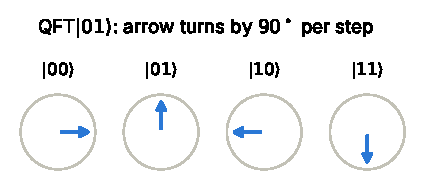
\includegraphics[width=0.45\textwidth]{clocks_qft1_2q}\\
  \raggedright\small
  Each amplitude drawn as a clock hand (CUDA-Q result). For $x = 1$ the hand turns $90^\circ$ from one $\ket y$ to
  the next; for $x = 2$ it turns $180^\circ$. \hl{The input $x$ sets the speed of rotation} --- a frequency.
\end{frame}

\begin{frame}{Three qubits: phase clocks}
  \centering
  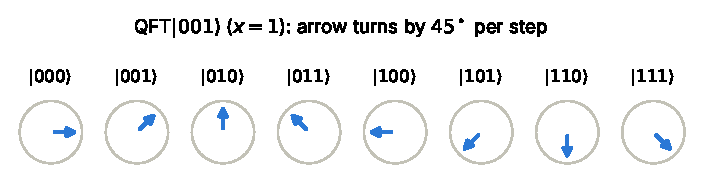
\includegraphics[width=0.85\textwidth]{clocks_qft1_3q}\\[3mm]
  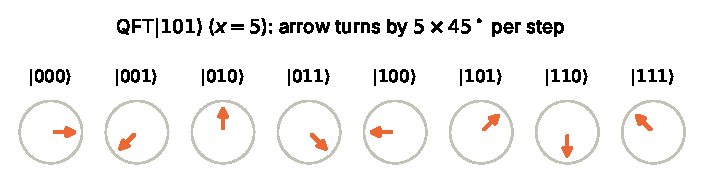
\includegraphics[width=0.85\textwidth]{clocks_qft5_3q}\\[2mm]
  \raggedright
  $M = 8$: the amplitude of $\ket y$ in $\mathrm{QFT}\ket x$ points at angle $360^\circ\cdot xy/8$.
  All arrows have the same length $1/\sqrt8$ --- only the \key{directions} encode $x$.
\end{frame}

\begin{frame}{Checking the numbers with CUDA-Q: $\mathrm{QFT}\ket{101}$}
  \begin{columns}[c]
    \begin{column}{0.55\textwidth}
      \centering\small
      \begin{tabular}{ccrrrr}
        \toprule
        $\ket y$ & $y$ & Re & Im & angle & $|\beta_y|^2$\\
        \midrule
        \qftfiverows
        \bottomrule
      \end{tabular}
    \end{column}
    \begin{column}{0.42\textwidth}
      \begin{itemize}
        \item Simulated with CUDA-Q (\texttt{cudaq.get\_state}).
        \item Angle $= 225^\circ\cdot y \bmod 360^\circ$, exactly $\omega^{5y}$ with $\omega = e^{i\pi/4}$.
        \item $0.3536 = 1/\sqrt8$, $\ 0.25 = \tfrac{1}{\sqrt8}\cos 45^\circ$.
        \item Every probability is $1/8$.
      \end{itemize}
    \end{column}
  \end{columns}
\end{frame}

\begin{frame}{Measuring $\mathrm{QFT}\ket{x}$ tells us nothing about $x$}
  \begin{columns}[c]
    \begin{column}{0.55\textwidth}
      \centering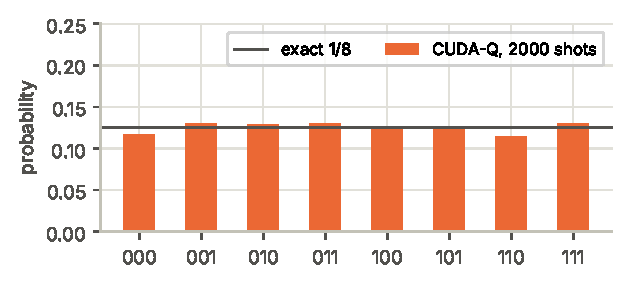
\includegraphics[width=\textwidth]{measure_qft5}\\
      \small $\mathrm{QFT}\ket{101}$ measured 2000 times with CUDA-Q
    \end{column}
    \begin{column}{0.42\textwidth}
      \[ P(y) = \Big|\frac{\omega^{xy}}{\sqrt M}\Big|^2 = \frac1M \quad\text{for every } y \]
      The histogram is \key{flat}, whatever $x$ is: the information sits in the phases, which a measurement does
      not show.
      \begin{alertblock}{Lesson}
        The QFT is useful when the input has \hl{structure} (e.g.\ a period); then the output has peaks (Part 6).
      \end{alertblock}
    \end{column}
  \end{columns}
\end{frame}

\begin{frame}{The QFT can be undone: the inverse QFT}
  \begin{itemize}
    \item The columns of $F_M$ are orthonormal (by the ``arrows cancel'' sum), so $F_M^\dagger F_M = I$:
      the QFT is \key{unitary}.
    \item The \key{inverse QFT} just flips the sign of the phase:
      \[ \mathrm{QFT}^{-1}\ket{y} = \frac{1}{\sqrt M}\sum_{x=0}^{M-1} e^{-2\pi i\,xy/M}\ket{x} \]
    \item Circuit: run the QFT circuit \hl{backwards} with all rotation angles negated.
  \end{itemize}
  \begin{block}{Why it matters}
    Most algorithms (phase estimation, Shor) use the \emph{inverse} QFT at the end to turn phases back into a bit
    string that can be measured.
  \end{block}
\end{frame}

% =====================================================================================
\section{Part 5: Building the circuit}
\begin{frame}{The key trick: the product formula}
  The $2^n$-term sum factorises into $n$ single-qubit states:
  \begin{block}{Product formula}
    \[ \begin{aligned}\mathrm{QFT}\ket{x_1x_2\dots x_n} = \frac{1}{\sqrt{2^n}}\,
       &\big(\ket0 + e^{2\pi i\,0.x_n}\ket1\big)\otimes
       \big(\ket0 + e^{2\pi i\,0.x_{n-1}x_n}\ket1\big)\\
       &\otimes\cdots\otimes
       \big(\ket0 + e^{2\pi i\,0.x_1x_2\dots x_n}\ket1\big)\end{aligned} \]
  \end{block}
  \begin{itemize}
    \item Every output qubit is a \key{phase state} $\tfrac{1}{\sqrt2}(\ket0 + e^{i\varphi}\ket1)$.
    \item Its angle is a \key{binary fraction} built from the last bits of $x$.
    \item No entanglement in the output of a basis state --- so it can be built qubit by qubit!
  \end{itemize}
  The next two slides prove it; you can skip the proof and trust the formula.
\end{frame}

\begin{frame}{Proof, step 1: split $y$ into its bits}
  Write $y = y_1y_2\dots y_n$, so $\dfrac{y}{2^n} = \dfrac{y_1}{2} + \dfrac{y_2}{4} + \dots + \dfrac{y_n}{2^n} = \displaystyle\sum_{l=1}^{n}\frac{y_l}{2^l}$. Then
  \[ e^{2\pi i\,xy/2^n} = \prod_{l=1}^{n} e^{2\pi i\,x\,y_l/2^l} \qquad (e^{a+b} = e^a e^b) \]
  Summing over all $y$ means summing over every bit $y_l\in\{0,1\}$ independently, so the sum becomes a product:
  \[ \mathrm{QFT}\ket x = \frac{1}{\sqrt{2^n}}\sum_{y_1=0}^{1}\cdots\sum_{y_n=0}^{1}\ \prod_{l=1}^{n} e^{2\pi i\,x y_l/2^l}\ket{y_l}
     = \frac{1}{\sqrt{2^n}}\bigotimes_{l=1}^{n}\Big(\ket0 + e^{2\pi i\,x/2^l}\ket1\Big) \]
  (For $y_l = 0$ the phase is 1, for $y_l = 1$ it is $e^{2\pi i\,x/2^l}$.)
\end{frame}

\begin{frame}{Proof, step 2: only the fractional part survives}
  Dividing $x$ by $2^l$ moves the binary point $l$ places to the left:
  \[ \frac{x}{2^l} = \underbrace{x_1\dots x_{n-l}}_{\text{integer}}\,.\,x_{n-l+1}\dots x_n \]
  The integer part is a whole number of turns, and $e^{2\pi i\cdot\text{integer}} = 1$, so
  \[ e^{2\pi i\,x/2^l} = e^{2\pi i\,0.x_{n-l+1}\dots x_n} . \]
  \begin{exampleblock}{Example $x = 5 = 101_2$}
    \centering
    \begin{tabular}{cccc}
      $l$ & $x/2^l$ & binary & phase factor\\
      \midrule
      1 & $2.5$ & $10.1_2$ & $e^{2\pi i\,0.1_2} = e^{i\pi} = -1$\\
      2 & $1.25$ & $1.01_2$ & $e^{2\pi i\,0.01_2} = e^{i\pi/2} = i$\\
      3 & $0.625$ & $0.101_2$ & $e^{2\pi i\,0.101_2} = e^{i5\pi/4}$
    \end{tabular}
  \end{exampleblock}
\end{frame}

\begin{frame}{What the output qubits look like for $x = 5$}
  \centering
  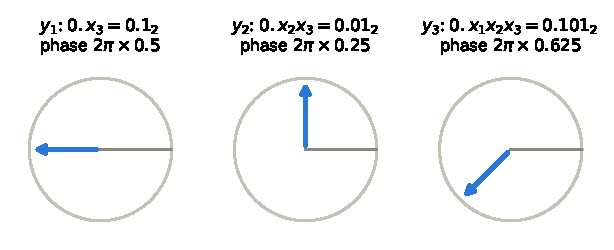
\includegraphics[width=0.82\textwidth]{qubit_phases_x5}\\[2mm]
  \raggedright
  \[ \mathrm{QFT}\ket{101} = \tfrac{1}{\sqrt8}\big(\ket0 - \ket1\big)\otimes\big(\ket0 + i\ket1\big)\otimes\big(\ket0 + e^{i5\pi/4}\ket1\big) \]
  Each output qubit is a clock hand on the ``equator''. Multiplying out the brackets gives back the 8 amplitudes
  $\omega^{5y}/\sqrt8$ from the CUDA-Q table.
\end{frame}

\begin{frame}{Ingredient 1: the Hadamard writes the first bit}
  Recall $H\ket{b} = \tfrac{1}{\sqrt2}(\ket0 + (-1)^b\ket1)$ and $(-1)^b = e^{i\pi b} = e^{2\pi i\,b/2} = e^{2\pi i\,0.b}$:
  \begin{block}{}
    \[ H\ket{x_j} = \tfrac{1}{\sqrt2}\big(\ket0 + e^{2\pi i\,0.x_j}\ket1\big) \]
  \end{block}
  \begin{itemize}
    \item After the Hadamard, the qubit is a phase state whose angle is $0.x_j$ in binary: $0^\circ$ if $x_j = 0$,
      $180^\circ$ if $x_j = 1$.
    \item We still need to add the \emph{following} bits: $0.x_j \to 0.x_jx_{j+1}\dots x_n$.
  \end{itemize}
\end{frame}

\begin{frame}{Ingredient 2: controlled rotations add the next bits}
  \begin{columns}[T]
    \begin{column}{0.52\textwidth}
      A controlled-$R_k$ with control $x_m$ multiplies the $\ket1$ part of the target by $e^{2\pi i/2^k}$ \emph{only if}
      $x_m = 1$, i.e.\ it adds $x_m/2^k$ to the phase fraction. Since $0.x_j + x_{j+1}/4 = 0.x_jx_{j+1}$:
      \[ \begin{aligned}
        & e^{2\pi i\,0.x_j}\\
        \xrightarrow{\ R_2,\ \text{control } x_{j+1}\ }\ & e^{2\pi i\,0.x_jx_{j+1}}\\
        \xrightarrow{\ R_3,\ \text{control } x_{j+2}\ }\ & e^{2\pi i\,0.x_jx_{j+1}x_{j+2}}\ \to\ \cdots
      \end{aligned} \]
    \end{column}
    \begin{column}{0.44\textwidth}
      \begin{block}{Recipe for qubit $j$}
        \begin{enumerate}
          \item Hadamard on qubit $j$
          \item $R_2$ controlled by qubit $j{+}1$
          \item $R_3$ controlled by qubit $j{+}2$
          \item \dots\ up to $R_{n-j+1}$ controlled by qubit $n$
        \end{enumerate}
        Result: $\tfrac{1}{\sqrt2}(\ket0 + e^{2\pi i\,0.x_j\dots x_n}\ket1)$
      \end{block}
    \end{column}
  \end{columns}
\end{frame}

\begin{frame}[fragile]{The 3-qubit QFT circuit}
  \centering
  \begin{quantikz}[row sep=0.45cm, column sep=0.35cm]
    \lstick{$\ket{x_1}$} & \gate{H} & \gate{R_2} & \gate{R_3} & \qw & \qw & \qw & \swap{2} & \rstick{$\ket0 + e^{2\pi i\,0.x_3}\ket1$}\qw\\
    \lstick{$\ket{x_2}$} & \qw & \ctrl{-1} & \qw & \gate{H} & \gate{R_2} & \qw & \qw & \rstick{$\ket0 + e^{2\pi i\,0.x_2x_3}\ket1$}\qw\\
    \lstick{$\ket{x_3}$} & \qw & \qw & \ctrl{-2} & \qw & \ctrl{-1} & \gate{H} & \targX{} & \rstick{$\ket0 + e^{2\pi i\,0.x_1x_2x_3}\ket1$}\qw
  \end{quantikz}\\[4mm]
  \raggedright
  \begin{itemize}
    \item Top wire: $H$, then $R_2$ (control $x_2$) and $R_3$ (control $x_3$) $\Rightarrow$ phase $0.x_1x_2x_3$.
    \item Middle wire: $H$, then $R_2$ (control $x_3$) $\Rightarrow$ phase $0.x_2x_3$. Bottom wire: $H$ $\Rightarrow$ $0.x_3$.
    \item The SWAP puts the qubits in the order of the product formula (normalisation $1/\sqrt8$ omitted).
  \end{itemize}
\end{frame}

\begin{frame}{Walk-through: $\ket{101}$ through the circuit}
  After its Hadamard each wire is a phase state $\tfrac{1}{\sqrt2}\big(\ket0 + e^{2\pi i f}\ket1\big)$; the table tracks the
  binary fraction $f$.\\[2mm]
  \centering\small
  \begin{tabular}{lccc}
    \toprule
    after gate & wire 1 & wire 2 & wire 3\\
    \midrule
    start & $\ket1$ & $\ket0$ & $\ket1$\\
    $H$ on wire 1 & $f = 0.1_2$ & $\ket0$ & $\ket1$\\
    $R_2$, control wire 2 ($=0$) & $f = 0.10_2$ (no change) & $\ket0$ & $\ket1$\\
    $R_3$, control wire 3 ($=1$) & $f = 0.101_2$ & $\ket0$ & $\ket1$\\
    $H$ on wire 2 & $\cdot$ & $f = 0.0_2$ & $\ket1$\\
    $R_2$, control wire 3 ($=1$) & $\cdot$ & $f = 0.01_2$ & $\ket1$\\
    $H$ on wire 3 & $\cdot$ & $\cdot$ & $f = 0.1_2$\\
    \midrule
    SWAP wires 1 and 3 & $0.1_2$: phase $-1$ & $0.01_2$: phase $i$ & $0.101_2$: phase $e^{i5\pi/4}$\\
    \bottomrule
  \end{tabular}\\[3mm]
  \raggedright\normalsize
  This is exactly the product formula for $x = 5$. Wires 2 and 3 are used as \key{controls before} they receive their
  own Hadamard --- that is why the order of the gates matters.
\end{frame}

\begin{frame}{Why the SWAPs at the end?}
  \begin{columns}[T]
    \begin{column}{0.52\textwidth}
      \begin{itemize}
        \item The circuit leaves qubit 1 with the phase $0.x_1x_2\dots x_n$ --- but the product formula wants that
          phase on the \key{last} qubit.
        \item The outputs come out in \hl{reversed order}.
        \item Fix: SWAP qubit 1 $\leftrightarrow$ $n$, 2 $\leftrightarrow$ $n{-}1$, \dots: $\lfloor n/2\rfloor$ swaps.
        \item Many algorithms skip the swaps and simply read the bits in reverse order (it is free).
      \end{itemize}
    \end{column}
    \begin{column}{0.44\textwidth}
      \begin{block}{A SWAP is 3 CNOTs}
        SWAP exchanges two qubits:
        $\ket{ab} \mapsto \ket{ba}$.\\[1mm]
        It can be built from three CNOTs with alternating directions.
      \end{block}
    \end{column}
  \end{columns}
\end{frame}

\begin{frame}[fragile]{The general $n$-qubit circuit}
  \centering
  \begin{quantikz}[row sep=0.32cm, column sep=0.26cm, wire types={q,q,n,q,q}]
    \lstick{$\ket{x_1}$} & \gate{H} & \gate{R_2} & \ \cdots\ & \gate{R_{n-1}} & \gate{R_n} & \qw & \ \cdots\ & \qw & \ \cdots\ & \qw & \qw & \qw & \swap{4} & \qw\\
    \lstick{$\ket{x_2}$} & \qw & \ctrl{-1} & \ \cdots\ & \qw & \qw & \gate{H} & \ \cdots\ & \gate{R_{n-1}} & \ \cdots\ & \qw & \qw & \qw & \qw & \qw\\
    \lstick{$\vdots$} & & & & & & & & & & & & & &\\
    \lstick{$\ket{x_{n-1}}$} & \qw & \qw & \ \cdots\ & \ctrl{-3} & \qw & \qw & \ \cdots\ & \qw & \ \cdots\ & \gate{H} & \gate{R_2} & \qw & \qw & \qw\\
    \lstick{$\ket{x_n}$} & \qw & \qw & \ \cdots\ & \qw & \ctrl{-4} & \qw & \ \cdots\ & \ctrl{-3} & \ \cdots\ & \qw & \ctrl{-1} & \gate{H} & \targX{} & \qw
  \end{quantikz}\\[3mm]
  \raggedright
  Qubit $j$ gets one Hadamard and $n - j$ controlled rotations $R_2, \dots, R_{n-j+1}$; then the order is reversed
  with SWAPs (only the outer pair is drawn).
\end{frame}

\begin{frame}{Counting gates: why the QFT is fast}
  \begin{columns}[c]
    \begin{column}{0.47\textwidth}
      \begin{itemize}
        \item Hadamards: $n$
        \item controlled rotations: $(n-1) + (n-2) + \dots + 1 = \dfrac{n(n-1)}{2}$
        \item SWAPs: $\lfloor n/2\rfloor$
      \end{itemize}
      \begin{block}{Total}
        $\approx n^2/2$ gates for $2^n$ amplitudes.
        $n = 15$: $15 + 105 + 7 = 127$ gates;\\
        $n = 30$: $480$ gates.
      \end{block}
    \end{column}
    \begin{column}{0.5\textwidth}
      \centering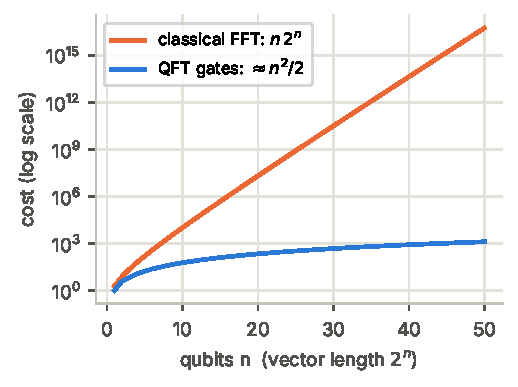
\includegraphics[width=\textwidth]{scaling}\\
      \small Exponential (FFT) vs.\ quadratic (QFT) growth
    \end{column}
  \end{columns}
\end{frame}

\begin{frame}{The approximate QFT}
  \begin{columns}[c]
    \begin{column}{0.5\textwidth}
      $R_k$ rotates by $360^\circ/2^k$ --- tiny for large $k$:
      \begin{itemize}
        \item $R_{10}$: $0.35^\circ$, $\ R_{15}$: $0.011^\circ$
        \item Real gates have errors larger than that anyway.
      \end{itemize}
      \begin{block}{Approximate QFT}
        Keep only $R_k$ with $k \le m$ ($m \approx \log_2 n + 2$). The result is almost identical, but needs only
        about $n\,m$ gates, i.e.\ $O(n\log n)$.
      \end{block}
    \end{column}
    \begin{column}{0.47\textwidth}
      \centering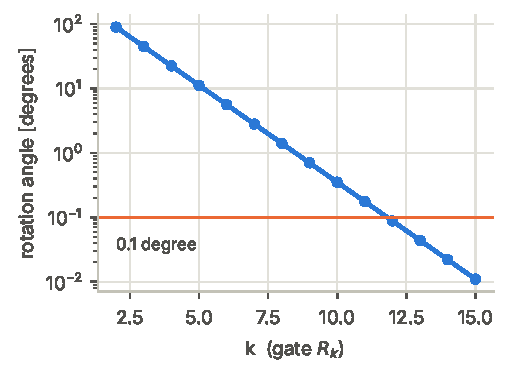
\includegraphics[width=\textwidth]{approx_angles}
    \end{column}
  \end{columns}
\end{frame}

% =====================================================================================
\section{Part 6: Examples --- finding periods}
\begin{frame}{Periodic states: the math}
  A state with period $r$ (dividing $M$) and offset $o$ uses $K = M/r$ basis states:
  \[ \ket\psi = \frac{1}{\sqrt K}\sum_{j=0}^{K-1}\ket{j\,r + o} \]
  Apply the QFT and collect the amplitude of $\ket y$:
  \[ \beta_y = \frac{1}{\sqrt{MK}}\sum_{j=0}^{K-1}\omega^{(jr+o)y} = \frac{\omega^{oy}}{\sqrt{MK}}\underbrace{\sum_{j=0}^{K-1} e^{2\pi i\,j\,ry/M}}_{= K \text{ if } ry/M \in \mathbb{Z}, \text{ else } 0} \]
  \begin{block}{Result}
    Only $y = 0, \tfrac{M}{r}, \tfrac{2M}{r}, \dots$ survive, each with probability $1/r$ --- the same pattern as the
    classical DFT example in Part 1.
  \end{block}
\end{frame}

\begin{frame}{Example: 4 qubits, period 4, offset 1}
  \centering
  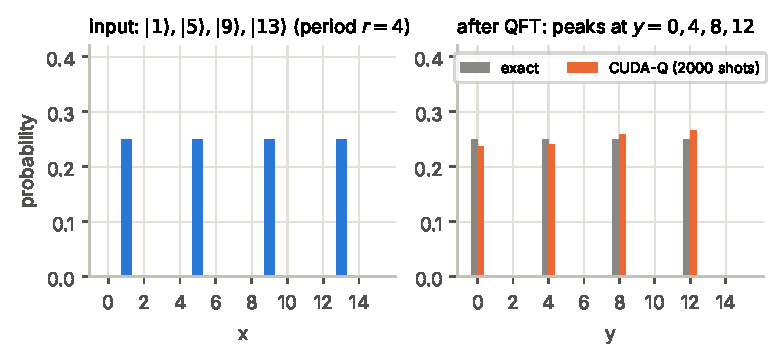
\includegraphics[width=0.86\textwidth]{periodic_4q}\\[0mm]
  \raggedright
  $M = 16$, $r = 4$: input $\tfrac12(\ket1 + \ket5 + \ket9 + \ket{13})$. Prediction: peaks at multiples of
  $16/4 = 4$, each with probability $1/4$. The CUDA-Q simulation (2000 shots) agrees; the small differences are
  shot noise ($\approx 1/\sqrt{2000}$).
\end{frame}

\begin{frame}{The offset hides in the phases}
  \begin{columns}[c]
    \begin{column}{0.5\textwidth}
      \centering
      \begin{tabular}{crcc}
        \toprule
        $y$ & $\beta_y$ (CUDA-Q) & $|\beta_y|^2$ & angle\\
        \midrule
        \periodicrows
        \bottomrule
      \end{tabular}
    \end{column}
    \begin{column}{0.46\textwidth}
      \begin{itemize}
        \item Theory: $\beta_y = \omega^{oy}/\sqrt r$ with $o = 1$: angles $360^\circ\cdot y/16$.
        \item Changing the offset $o$ only rotates these phases --- the \key{probabilities do not change}.
        \item This ``shift invariance'' is why the QFT finds the period no matter where the pattern starts.
      \end{itemize}
    \end{column}
  \end{columns}
\end{frame}

\begin{frame}{When the period does not divide $M$: leakage}
  \centering
  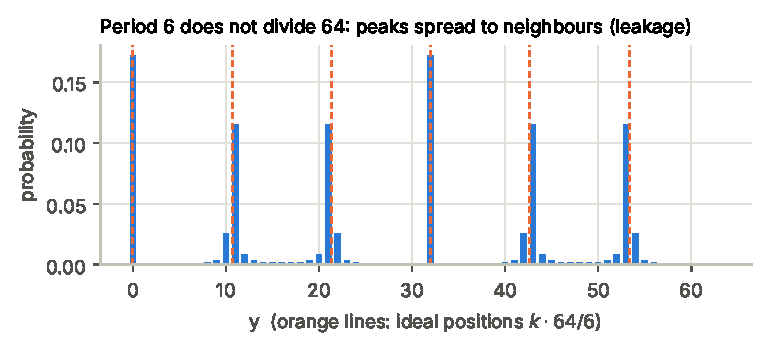
\includegraphics[width=0.8\textwidth]{leakage_6q}\\[0mm]
  \raggedright
  $n = 6$ ($M = 64$), period $r = 6$: $64/6 \approx 10.67$ is not an integer. The arrows no longer cancel
  perfectly: the peaks sit \key{near} $k\cdot 64/6$ and spread to neighbouring $y$. More qubits make them
  sharper; Shor's algorithm handles this with \hl{continued fractions} (two slides ahead).
\end{frame}

\begin{frame}{A bigger simulation: 15 qubits with CUDA-Q}
  \centering
  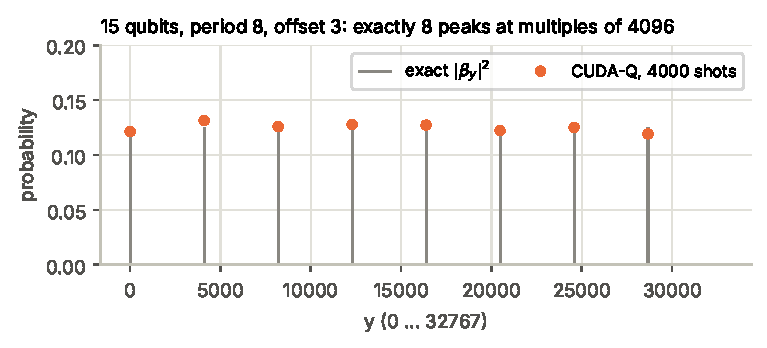
\includegraphics[width=0.84\textwidth]{qft_15q}\\[0mm]
  \raggedright
  $M = 32\,768$ amplitudes, period 8, offset 3 (the default example of \texttt{QFT.ipynb}). CUDA-Q's state agrees with
  NumPy's FFT with fidelity \fidfifteen{} (largest amplitude error \maxerrfifteen). With 4000 shots we only ever see
  the 8 peaks --- the other 32\,760 outcomes have probability zero.
\end{frame}

\begin{frame}{From a measured peak to the period}
  A measurement gives one $y$ with $\dfrac{y}{M} \approx \dfrac{k}{r}$ for some unknown integer $k$.
  \begin{exampleblock}{Example ($M = 64$, true period $r = 6$)}
    We measure $y = 11$: $\ 11/64 = 0.171875$.\\
    Best fraction with a small denominator: $1/6 = 0.1667$ $\Rightarrow$ guess $r = 6$. \checkmark\\[1mm]
    We measure $y = 21$: $\ 21/64 = 0.328 \approx 1/3$ $\Rightarrow$ $r = 3$ is only a divisor of 6 --- measure again.
  \end{exampleblock}
  \begin{itemize}
    \item The ``best fraction'' comes from the \key{continued-fraction expansion} (in Python:
      \texttt{Fraction(11, 64).limit\_denominator(10)}).
    \item A few shots are enough to find $r$ with high probability.
    \item In \key{Shor's algorithm}, $r$ is the period of $a^x \bmod N$ and it reveals the factors of $N$.
  \end{itemize}
\end{frame}

% =====================================================================================
\section{Part 7: The QFT in practice}
\begin{frame}{Where the QFT is used}
  \begin{columns}[T]
    \begin{column}{0.48\textwidth}
      \begin{block}{Quantum phase estimation}
        Measures the eigenvalue $e^{2\pi i\varphi}$ of a unitary: the core of quantum chemistry (molecular energies)
        and of HHL (linear systems).
      \end{block}
      \begin{block}{Shor's factoring algorithm}
        Finds the period of $a^x \bmod N$; breaks RSA on a large fault-tolerant quantum computer.
      \end{block}
    \end{column}
    \begin{column}{0.48\textwidth}
      \begin{block}{Quantum arithmetic}
        Adding numbers ``in Fourier space'' needs only phase rotations (Draper adder).
      \end{block}
      \begin{block}{Hidden structure}
        Hidden subgroup problems, period finding in general.
      \end{block}
      \small The notebooks \texttt{Shor.ipynb} and \texttt{HHL.ipynb} in this repository both contain an inverse QFT.
    \end{column}
  \end{columns}
\end{frame}

\begin{frame}[fragile]{Inside phase estimation: the inverse QFT at work}
  \centering
  \begin{quantikz}[row sep=0.3cm, column sep=0.38cm]
    \lstick{$\ket0$} & \gate{H} & \qw & \qw & \ctrl{3} & \gate[3]{\mathrm{QFT}^{-1}} & \meter{}\\
    \lstick{$\ket0$} & \gate{H} & \qw & \ctrl{2} & \qw & & \meter{}\\
    \lstick{$\ket0$} & \gate{H} & \ctrl{1} & \qw & \qw & & \meter{}\\
    \lstick{$\ket u$} & \qw & \gate{U} & \gate{U^2} & \gate{U^4} & \qw & \qw
  \end{quantikz}\\[3mm]
  \raggedright
  \begin{itemize}
    \item $U\ket u = e^{2\pi i\varphi}\ket u$. The controlled powers $U^{2^j}$ write the phases $e^{2\pi i\,2^j\varphi}$
      onto the top qubits --- exactly the pattern of the product formula.
    \item The inverse QFT turns this into the bit string $\varphi \approx 0.\varphi_1\varphi_2\varphi_3$, which we measure.
  \end{itemize}
\end{frame}

\begin{frame}{Limits: what the QFT does \emph{not} do}
  \begin{itemize}
    \item \key{No direct read-out}: the $2^n$ results are amplitudes. One shot gives one bit string; estimating all
      probabilities needs $\sim 2^n$ shots, and phases need even more. Useful algorithms only need a few peaks.
    \item \key{Input preparation}: loading an arbitrary list of $2^n$ numbers into a quantum state is itself expensive.
      The speed-up only pays off when the algorithm prepares the input (as in Shor or phase estimation).
    \item \key{Precision and noise}: tiny rotation angles and $\approx n^2/2$ gates make the QFT sensitive to gate errors
      --- see \texttt{Noise\_Simulation.ipynb}; the approximate QFT helps.
    \item \key{Simulation}: a classical simulator stores all $2^n$ amplitudes, so simulations stop at $\approx 30$--$45$
      qubits even on large GPU clusters.
  \end{itemize}
\end{frame}

\begin{frame}[fragile]{The QFT in CUDA-Q (from \texttt{QFT.ipynb})}
  \begin{columns}[T]
    \begin{column}{0.58\textwidth}
\begin{lstlisting}
import cudaq, numpy as np

@cudaq.kernel
def qft(qubits: cudaq.qview):
    n = qubits.size()
    for j in range(n):
        h(qubits[j])                       # Hadamard
        for k in range(j + 1, n):          # R_(k-j+1)
            r1.ctrl(np.pi / 2**(k - j),
                    qubits[k], qubits[j])
    for j in range(n // 2):                # reverse order
        swap(qubits[j], qubits[n - 1 - j])

@cudaq.kernel
def demo():
    q = cudaq.qvector(3)
    x(q[0]); x(q[2])                       # |101> = |5>
    qft(q)

print(cudaq.draw(demo))
state = cudaq.get_state(demo)
\end{lstlisting}
    \end{column}
    \begin{column}{0.4\textwidth}
      \begin{itemize}
        \item \texttt{r1(angle)} $= \mathrm{diag}(1, e^{i\cdot\text{angle}})$, so \texttt{r1}$(\pi/2^{k-j}) = R_{k-j+1}$.
        \item \texttt{.ctrl(c, t)} makes it controlled.
        \item \texttt{cudaq.get\_state} returns the $2^n$ amplitudes; \texttt{cudaq.sample} measures.
        \item Note: \texttt{get\_state} lists amplitudes with qubit 0 as the \emph{least} significant bit; the
          notebook converts this for you.
      \end{itemize}
    \end{column}
  \end{columns}
\end{frame}

\begin{frame}{Try it yourself: \texttt{QFT.ipynb}}
  \begin{columns}[T]
    \begin{column}{0.5\textwidth}
      \begin{enumerate}
        \item Install: \texttt{pip install cudaq numpy scipy matplotlib psutil}
        \item Open \texttt{QFT.ipynb} and run all cells.
        \item Change only Section 3:
          \begin{itemize}
            \item \texttt{N\_QUBITS} (default 15)
            \item \texttt{INITIAL\_STATE}: \texttt{"periodic"}, \texttt{"basis"}, \texttt{"random"}, \texttt{"custom"}
            \item \texttt{PERIOD}, \texttt{OFFSET}
            \item \texttt{BACKEND}: \texttt{"cpu"} or \texttt{"gpu"}
          \end{itemize}
      \end{enumerate}
    \end{column}
    \begin{column}{0.46\textwidth}
      \begin{block}{Experiments}
        \begin{itemize}
          \item \texttt{PERIOD = 6}: see leakage
          \item \texttt{INITIAL\_STATE = "basis"}: a flat histogram, information only in the phases
          \item \texttt{N\_QUBITS = 25} on a GPU: compare the execution time with the CPU
        \end{itemize}
      \end{block}
      The notebook compares every result with NumPy's FFT and reports time and memory.
    \end{column}
  \end{columns}
\end{frame}

% =====================================================================================
\section{Part 8: Practice and summary}
\begin{frame}{Exercises}
  \begin{enumerate}
    \item Compute $\mathrm{QFT}\ket{11}$ for two qubits ($x = 3$).
    \item What is $\mathrm{QFT}\ket{000}$? What do you measure?
    \item For $x = 3 = 011_2$ on three qubits, give the phase of every output qubit (product formula).
    \item How many gates does the QFT on $n = 10$ qubits need (including SWAPs)?
    \item A 5-qubit state has period 8. Where are the peaks after the QFT, and how likely is each one?
    \item Why can't we read out all $2^n$ Fourier coefficients efficiently?
    \item Bonus: show that $F_4$ applied twice maps $\ket{x}$ to $\ket{-x \bmod 4}$.
  \end{enumerate}
\end{frame}

\begin{frame}{Answers}
  \small
  \begin{enumerate}
    \item Column $x = 3$ of $F_4$: $\tfrac12\big(\ket{00} - i\ket{01} - \ket{10} + i\ket{11}\big)$.
    \item $\tfrac{1}{\sqrt8}\sum_y\ket y$ --- all phases are 1 ($x = 0$). Every outcome has probability $1/8$.
    \item $x_1x_2x_3 = 011$: $0.x_3 = 0.1_2 \to 180^\circ$; $\ 0.x_2x_3 = 0.11_2 = 3/4 \to 270^\circ$;
      $\ 0.x_1x_2x_3 = 0.011_2 = 3/8 \to 135^\circ$.
    \item $10 + 45 + 5 = 60$ gates.
    \item $M = 32$, $M/r = 4$: peaks at $y = 0, 4, 8, \dots, 28$; 8 peaks with probability $1/8$ each.
    \item Each shot returns one bit string; estimating $2^n$ probabilities needs about $2^n$ shots (and the phases are
      not visible in a measurement at all).
    \item $F_4^2\ket x = \tfrac14\sum_{y,z} i^{xy} i^{yz}\ket z = \sum_z\big(\tfrac14\sum_y i^{y(x+z)}\big)\ket z$; the
      inner sum is 1 only if $x + z \equiv 0 \pmod 4$, so the result is $\ket{-x \bmod 4}$.
  \end{enumerate}
\end{frame}

\begin{frame}{Summary}
  \begin{columns}[T]
    \begin{column}{0.55\textwidth}
      \begin{itemize}
        \item The Fourier transform changes the view from \key{time} to \key{frequency}; periods become peaks.
        \item The QFT applies the DFT to the $2^n$ \key{amplitudes} of an $n$-qubit state:
          $\ket x \mapsto \tfrac{1}{\sqrt M}\sum_y \omega^{xy}\ket y$.
        \item The \key{product formula} turns it into one phase state per qubit, with angles given by
          \key{binary fractions} of $x$.
        \item Circuit: \key{Hadamards + controlled rotations + SWAPs}, only $\approx n^2/2$ gates.
        \item The output is in the amplitudes: useful when we only need a few \key{peaks}, e.g.\ a period.
      \end{itemize}
    \end{column}
    \begin{column}{0.42\textwidth}
      \begin{block}{Further reading}
        \small
        \begin{itemize}
          \item M.\,A.\ Nielsen, I.\,L.\ Chuang, \emph{Quantum Computation and Quantum Information}, Chapter 5
          \item D.\ Coppersmith, \emph{An approximate Fourier transform useful in quantum factoring} (1994)
          \item NVIDIA CUDA-Q documentation
          \item This repository: \texttt{QFT.ipynb}, \texttt{Shor.ipynb}, \texttt{HHL.ipynb}
        \end{itemize}
      \end{block}
    \end{column}
  \end{columns}
\end{frame}

\end{document}
